% Chapter where we present the results.

\chapter{Results}
\label{ch:results}

In Chapter \ref{ch:methods} we discussed a general solution to the protoboard
layout problem, and various alternatives that can be used in implementing the
solution. Figure \ref{fig:alternatives} presents the alternatives in a structured
way. Here, we will explore these alternatives and compare them quantitatively.
This section will provide data that is useful in comparing the alternatives, and
the data will be discussed in detail in Chapter \ref{ch:discussion}.

\begin{figure}[H]
\Tree [.{All Alternatives}
    [{Distance} {Block} ].Placement !\qsetw{4cm}
    [{All}
     [I D ].{Node}
     [I D ].{Pair} ].Wiring !\qsetw{4cm}
    [{Component} {Wire} ].Resistors !\qsetw{4cm}
    [$A*$ {Best First} ].Search ]
\label{fig:alternatives}
\caption{All possible alternatives to the algorithm.}
\end{figure}

As comparing all $40$ possible implementations of the algorithm is tedious, we
will compare the alternatives for each aspect of the algorithm while holding
other aspects fixed. Hence, we will carryout the following comparisons:

\begin{enumerate}
\item Placement: Distance vs. Blocking. Wiring method will be per-pair,
decreasing, resistors will be treated as components, and we will use $A*$.
\item Wiring: All pairs vs. Per-node, decreasing vs. Per-node, increasing vs.
Per-pair, decreasing vs. Per-pair, increasing. Placement method will be
blocking, resistors will be treated as components, and we will use $A*$.
\item Resistor treatment: As components vs. As wires. Placement method will be
blocking, wiring method will be per-pair, decreasing, and we will use $A*$.
\item Search: $A*$ vs. Best First. Placement method will be blocking, wiring
method will be per-pair, decreasing, and resistors will be treated as components.
\end{enumerate}

The data to compare the alternatives is gathered as described in Chapter
\ref{ch:methods}. We run the algorithm on $4425$ randomly generated schematics
of varying complexities. The algorithm is run $10$ times on each schematic.

In comparing alternatives, there are $3$ items we will consider:
\begin{enumerate}
\item Which alternative is the most successful?
\item Which alternative, when successful, takes the least amount of time?
\item Which alternative, when successful, produces the best layouts?
\end{enumerate}

In comparing success, we will look at bar graphs of the number of successes on
each of the $4425$ schematic out of the $10$ runs. We will also look at tables
that provide the same data in more detail. To get an understanding of how the
success rates vary with complexity, we will look at plots of circuit complexity
versus success rate, where our measure of circuit complexity will be the number
of pins in the circuit as discussed in Chapter \ref{ch:methods} (TODO: this is
currently not done, be sure to give a histogram of numbers of pins in the
circuits).

In comparing success time, we will look at CPU time spent on the wiring step, as
the placement step has much less variability. We will look at plots of circuit
complexity versus wiring times to do the comparisons.

In comparing the goodness of layouts, we will compare numbers of wires, total
lengths of wires, and numbers of wire crosses as functions of circuit complexity.

Below we will present the data for each of the comparisons outlined above. Note
that in all figures that follow, error bars indicate $1.96$ times the
standard error.

Discussion of these results will follow in Chapter \ref{ch:discussion}.

\section{Comparing placement methods}
\label{sec:compare_placement}

\begin{figure}[H]
\begin{center}
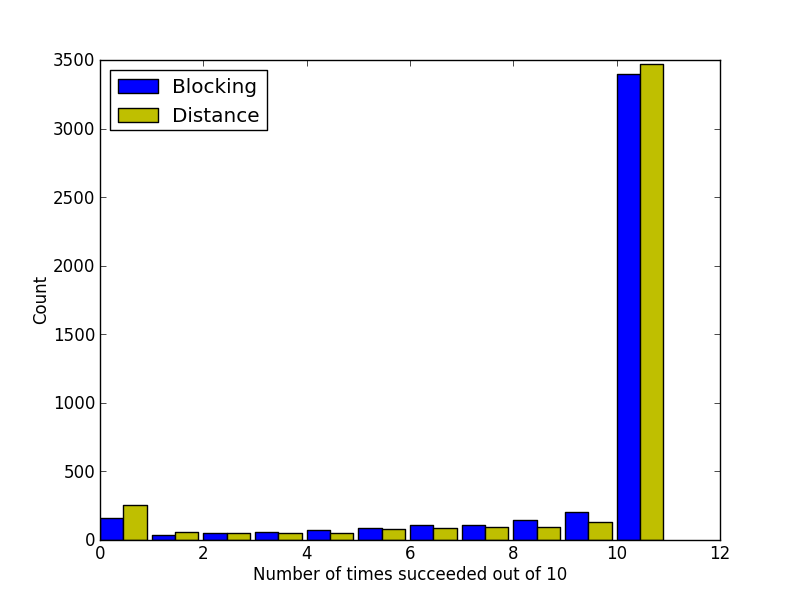
\includegraphics[width=\textwidth]{Images/placement_success_comparison.png}
\caption{Placement method comparison: success rates.}
\label{fig:placement_success}
\end{center}
\end{figure}

\begin{table}[H]
\begin{center}
\begin{singlespace}
\begin{tabular}{|c||c|c|c|c|c|c|c|c|c|c|c|}
\hline
 & \multicolumn{11}{|c|}{Number of times succeeded out of $10$} \\
\hline
 & 0 & 1 & 2 & 3 & 4 & 5 & 6 & 7 & 8 & 9 & 10 \\
\hline\hline
Blocking & $162$ & $38$ & $51$ & $57$ & $72$ & $85$ & $109$ & $106$ & $144$ & $203$ & $3398$ \\
 & $0.04$ & $0.01$ & $0.01$ & $0.01$ & $0.02$ & $0.02$ & $0.02$ & $0.02$ & $0.03$ & $0.05$ & $0.77$ \\
\hline
 Distance & $258$ & $55$ & $54$ & $50$ & $52$ & $77$ & $86$ & $97$ & $93$ & $130$ & $3473$ \\
  & $0.06$ & $0.01$ & $0.01$ & $0.01$ & $0.01$ & $0.02$ & $0.02$ & $0.02$ & $0.02$ & $0.03$ & $0.78$ \\
\hline
\end{tabular}
\end{singlespace}
\end{center}
\label{tb:placement_success}
\caption{Placement method comparison: success rates.}
\end{table}

\begin{figure}[H]
\begin{center}
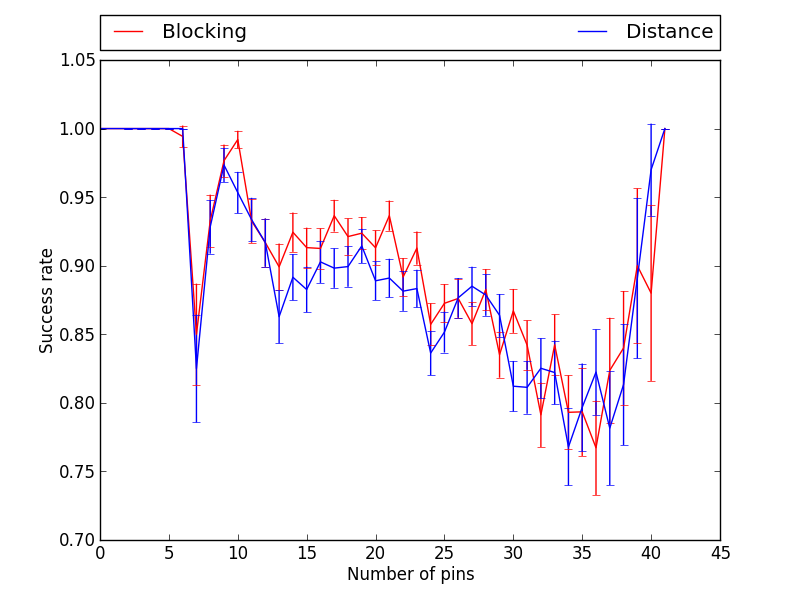
\includegraphics[width=\textwidth]{Images/placement_success_trend_comparison.png}
\caption{Placement method comparison: success rate trends.}
\label{fig:placement_success_trend}
\end{center}
\end{figure}

\begin{figure}[H]
\begin{center}
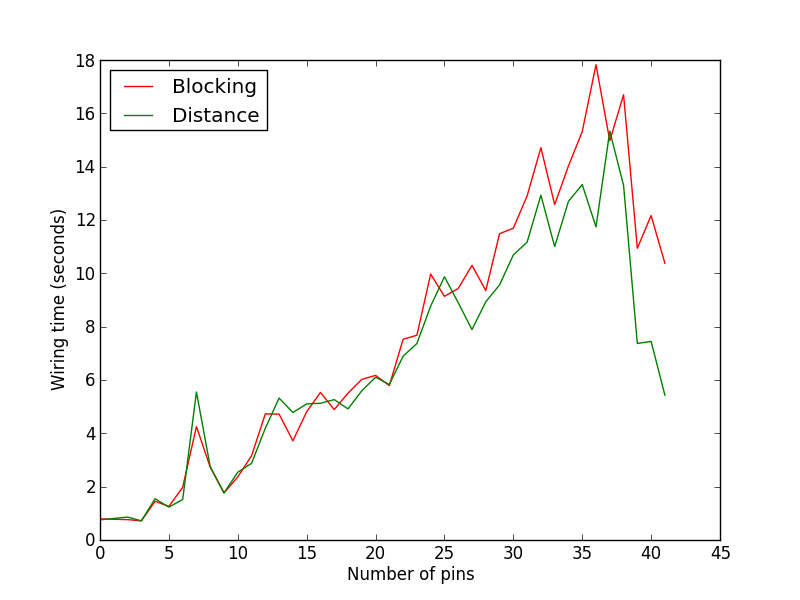
\includegraphics[width=\textwidth]{Images/placement_time_trend_comparison.png}
\caption{Placement method comparison: wiring time trends.}
\label{fig:placement_time_trend}
\end{center}
\end{figure}

\begin{figure}
\begin{center}
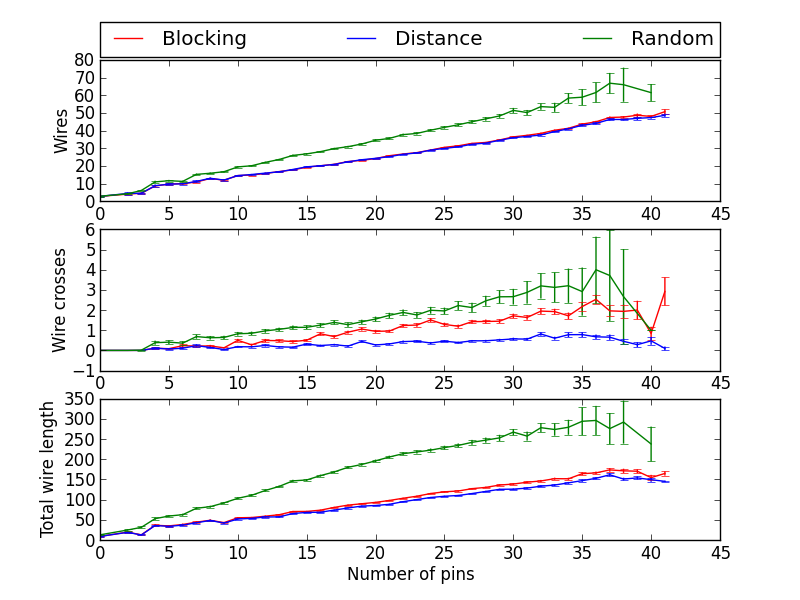
\includegraphics[width=\textwidth]{Images/placement_quality_trend_comparison.png}
\caption{Placement method comparison: layout quality trends.}
\label{fig:placement_quality_trend}
\end{center}
\end{figure}

\section{Comparing wiring methods}

\begin{figure}[H]
\begin{center}
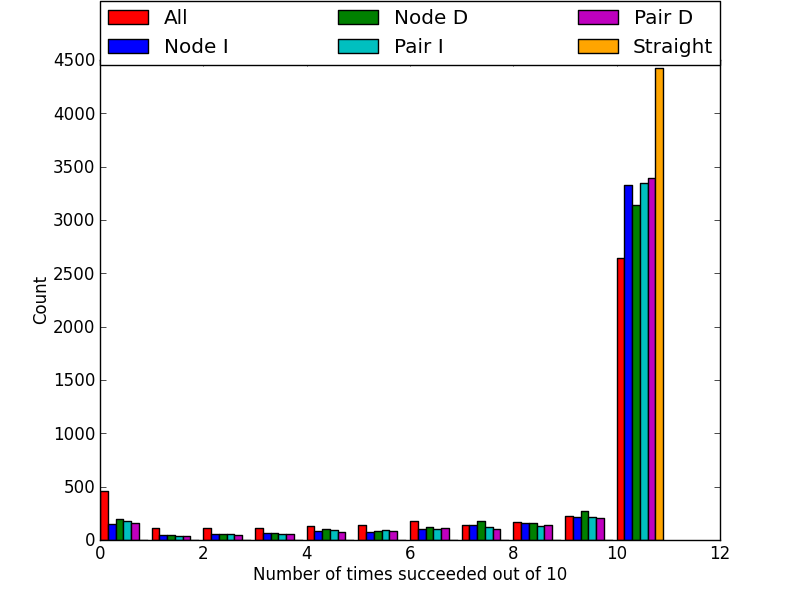
\includegraphics[width=\textwidth]{Images/wiring_success_comparison.png}
\caption{Wiring method comparison: success rates.}
\label{fig:wiring_success}
\end{center}
\end{figure}

\begin{table}[H]
\begin{center}
\begin{singlespace}
\begin{tabular}{|c||c|c|c|c|c|c|c|c|c|c|c|}
\hline
 & \multicolumn{11}{|c|}{Number of times succeeded out of $10$} \\
\hline
 & 0 & 1 & 2 & 3 & 4 & 5 & 6 & 7 & 8 & 9 & 10 \\
\hline\hline
All & $458$ & $114$ & $111$ & $112$ & $127$ & $145$ & $177$ & $139$ & $172$ & $227$ & $2643$ \\
 & $0.10$ & $0.03$ & $0.03$ & $0.03$ & $0.03$ & $0.03$ & $0.04$ & $0.03$ & $0.04$ & $0.05$ & $0.60$ \\
\hline
 Node D & $195$ & $50$ & $58$ & $66$ & $104$ & $83$ & $125$ & $176$ & $162$ & $268$ & $3138$ \\
  & $0.04$ & $0.01$ & $0.01$ & $0.01$ & $0.02$ & $0.02$ & $0.03$ & $0.04$ & $0.04$ & $0.06$ & $0.71$ \\
\hline
  Node I & $154$ & $50$ & $55$ & $62$ & $85$ & $71$ & $106$ & $141$ & $156$ & $217$ & $3328$ \\
   & $0.03$ & $0.01$ & $0.01$ & $0.01$ & $0.02$ & $0.02$ & $0.02$ & $0.03$ & $0.04$ & $0.05$ & $0.75$ \\
\hline
   Pair D & $162$ & $38$ & $51$ & $57$ & $72$ & $85$ & $109$ & $106$ & $144$ & $203$ & $3398$ \\
    & $0.04$ & $0.01$ & $0.01$ & $0.01$ & $0.02$ & $0.02$ & $0.02$ & $0.02$ & $0.03$ & $0.05$ & $0.77$ \\
\hline
    Pair I & $177$ & $40$ & $59$ & $54$ & $91$ & $92$ & $100$ & $118$ & $132$ & $212$ & $3350$ \\
     & $0.04$ & $0.01$ & $0.01$ & $0.01$ & $0.02$ & $0.02$ & $0.02$ & $0.03$ & $0.03$ & $0.05$ & $0.76$ \\
\hline
\end{tabular}
\end{singlespace}
\end{center}
\label{tb:wiring_success}
\caption{Wiring method comparison: success rates.}
\end{table}

\begin{figure}[H]
\begin{center}
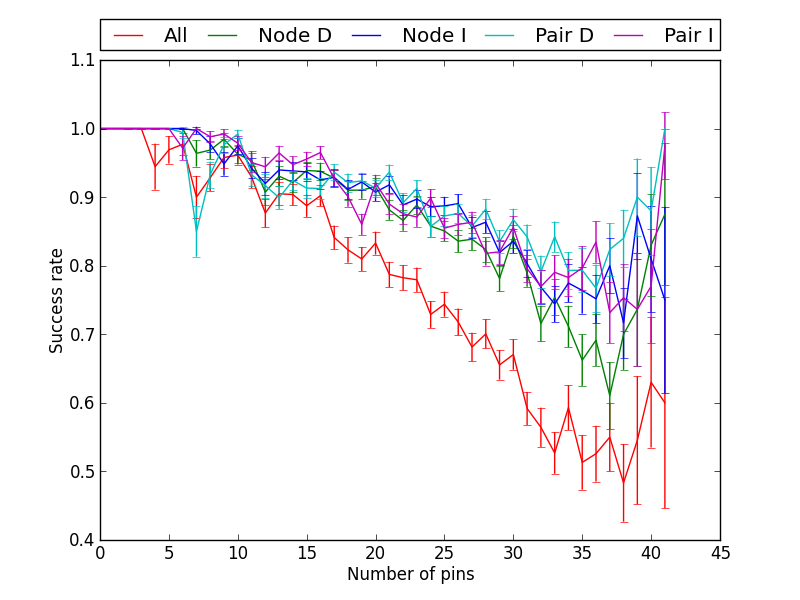
\includegraphics[width=\textwidth]{Images/wiring_success_trend_comparison.png}
\caption{Wiring method comparison: success rate trends.}
\label{fig:wiring_success_trend}
\end{center}
\end{figure}

\begin{figure}[H]
\begin{center}
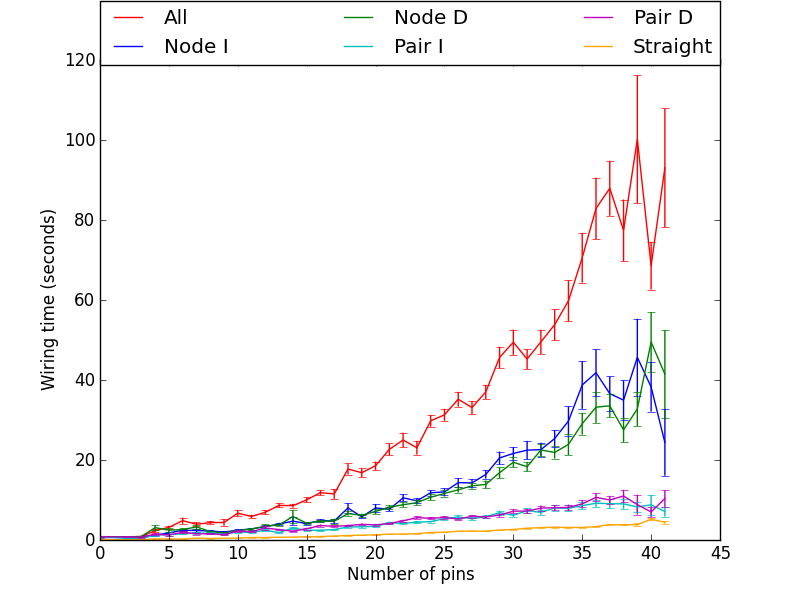
\includegraphics[width=\textwidth]{Images/wiring_time_trend_comparison.png}
\caption{Wiring method comparison: wiring time trends.}
\label{fig:wiring_time_trend}
\end{center}
\end{figure}

\begin{figure}
\begin{center}
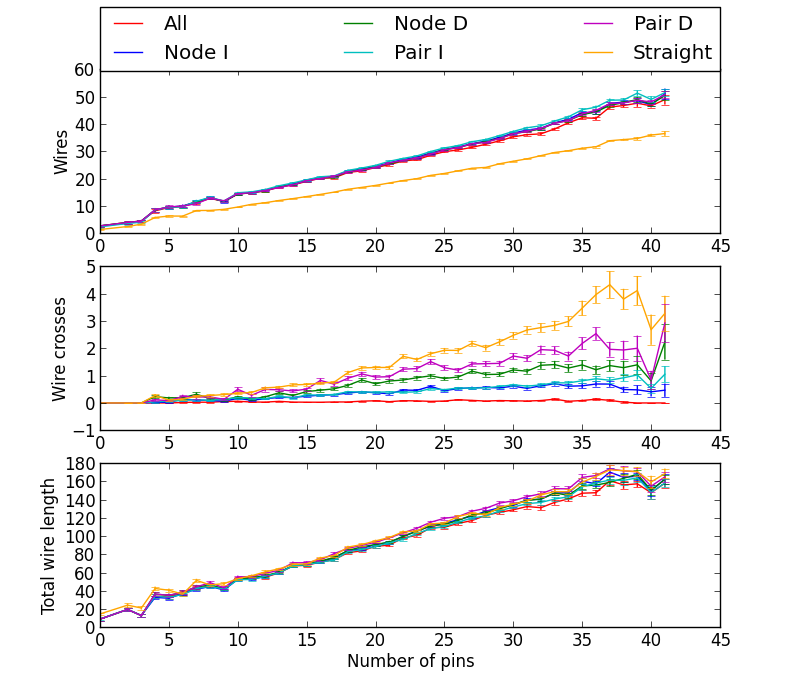
\includegraphics[width=\textwidth]{Images/wiring_quality_trend_comparison.png}
\caption{Wiring method comparison: layout quality trends.}
\label{fig:wiring_quality_trend}
\end{center}
\end{figure}

\section{Comparing resistor treatments}

\section{Comparing search methods}

\begin{figure}[H]
\begin{center}
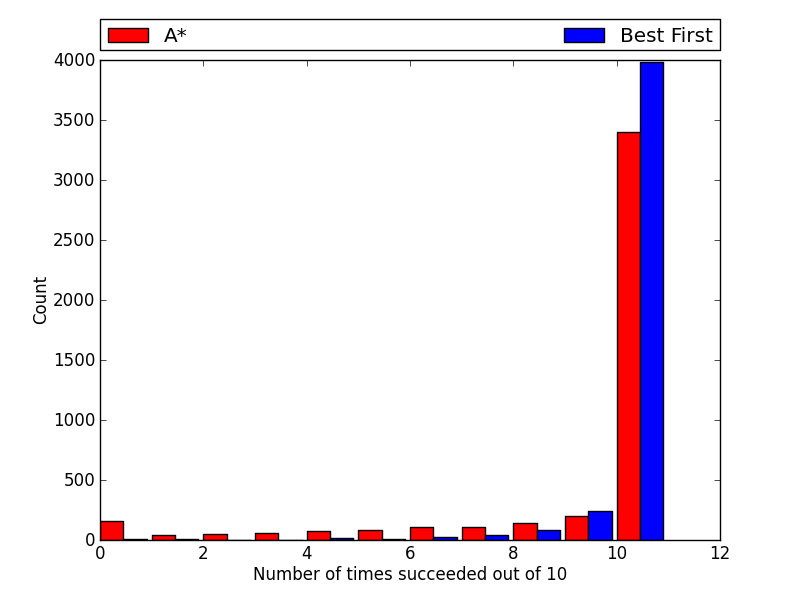
\includegraphics[width=\textwidth]{Images/search_success_comparison.png}
\caption{Search method comparison: success rates.}
\label{fig:search_success}
\end{center}
\end{figure}

\begin{table}[H]
\begin{center}
\begin{singlespace}
\begin{tabular}{|c||c|c|c|c|c|c|c|c|c|c|c|}
\hline
 & \multicolumn{11}{|c|}{Number of times succeeded out of $10$} \\
\hline
 & 0 & 1 & 2 & 3 & 4 & 5 & 6 & 7 & 8 & 9 & 10 \\
\hline\hline
$A*$ & $162$ & $38$ & $51$ & $57$ & $72$ & $85$ & $109$ & $106$ & $144$ & $203$ & $3398$ \\
 & $0.04$ & $0.01$ & $0.01$ & $0.01$ & $0.02$ & $0.02$ & $0.02$ & $0.02$ & $0.03$ & $0.05$ & $0.77$ \\
\hline
 Best First & $6$ & $5$ & $2$ & $1$ & $13$ & $10$ & $29$ & $45$ & $84$ & $245$ & $3985$ \\
  & $0.00$ & $0.00$ & $0.00$ & $0.00$ & $0.00$ & $0.00$ & $0.01$ & $0.01$ & $0.02$ & $0.06$ & $0.90$ \\
\hline
\end{tabular}
\end{singlespace}
\end{center}
\label{tb:search_success}
\caption{Search method comparison: success rates.}
\end{table}

\begin{figure}[H]
\begin{center}
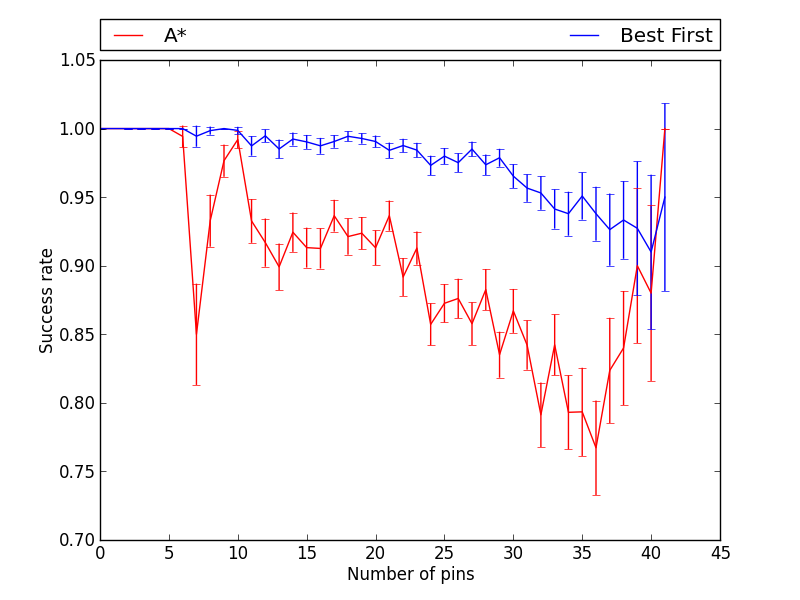
\includegraphics[width=\textwidth]{Images/search_success_trend_comparison.png}
\caption{Search method comparison: success rate trends.}
\label{fig:search_success_trend}
\end{center}
\end{figure}

\begin{figure}[H]
\begin{center}
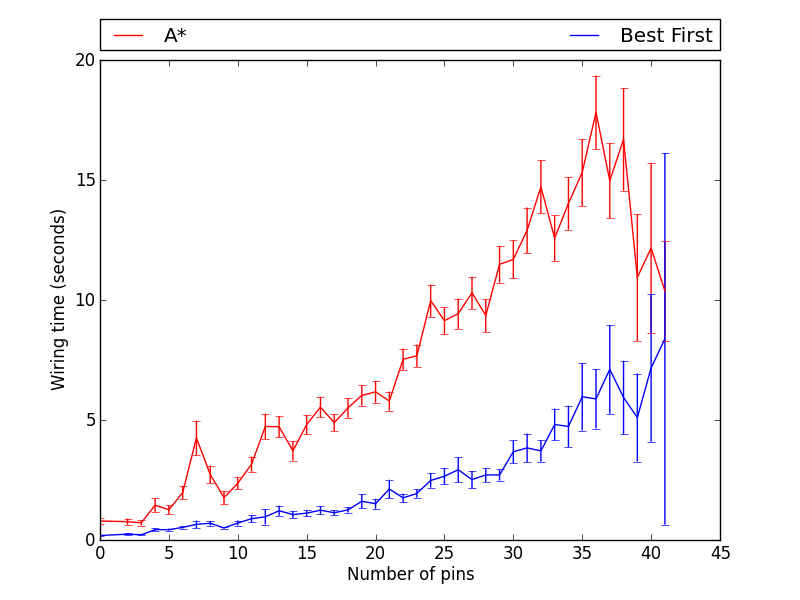
\includegraphics[width=\textwidth]{Images/search_time_trend_comparison.png}
\caption{Search method comparison: wiring time trends.}
\label{fig:search_time_trend}
\end{center}
\end{figure}

\begin{figure}
\begin{center}
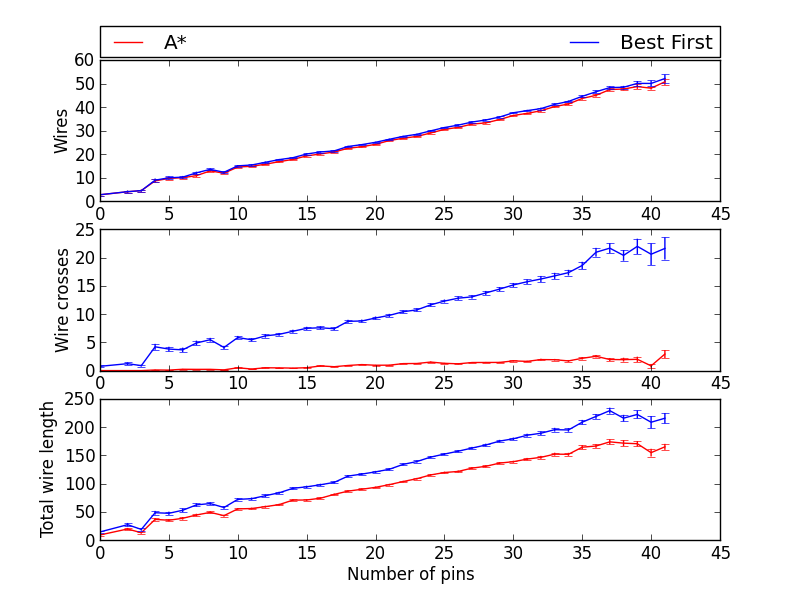
\includegraphics[width=\textwidth]{Images/search_quality_trend_comparison.png}
\caption{Search method comparison: layout quality trends.}
\label{fig:search_quality_trend}
\end{center}
\end{figure}

\section{Putting them all together}

\section{Exemplars}
